\documentclass[../main/main.tex]{subfiles}

\begin{document}
	
	\section{Optimaler Transport und Wassersteinmetriken}
	
	Wir orientieren uns an \cite{Villani.2009}.
	
	\subsection{Kopplungen}
	
	\begin{Definition}[Kopplung]
		Seien $\X$, $\Y$ topologische Räume und $A \subseteq \Probmeasures{\X}$, $B \subseteq \Probmeasures{\Y}$. Wir definieren dann
		\[ \Pi(A, B) \; \defby \; \setcomp{\pi \in \Probmeasures{\X \times \Y}}{\pi(\cdot \times \Y) \in A \quad \text{und} \quad \pi(\X \times \cdot) \in B} \text{.}\]
		Für $\mu \in \Probmeasures{\X}$ und $\nu \in \Probmeasures{\Y}$ definieren wir außerdem $\Pi(\mu, \nu) \; \defby \; \Pi(\set{\mu}, \set{\nu})$ und nennen die
		Elemente von $\Pi(\mu, \nu)$ \emph{Kopplungen} von $\mu$ und $\nu$ oder auch \emph{Transportpläne} zwischen $\mu$ und $\nu$.
	\end{Definition}

	\begin{Hilfssatz}
		\label{lem:couplingsproperties}
		Seien $\X$, $\Y$ polnische Räume und $A \subseteq \Probmeasures{\X}$ sowie $B \subseteq \Probmeasures{\Y}$. Dann gelten die folgenden Implikationen:
		\begin{enumeratethm}
			\item Sind $A$ und $B$ straff, so ist auch $\Pi(A, B) \subseteq \Probmeasures{\X \times \Y}$ straff.
			\item Sind $A$ und $B$ abgeschlossen, so ist auch $\Pi(A, B) \subseteq \Probmeasures{\X \times \Y}$ abgeschlossen.
			\item Sind $A$ und $B$ kompakt, so ist auch $\Pi(A, B) \subseteq \Probmeasures{\X \times \Y}$ kompakt.
		\end{enumeratethm}
	\end{Hilfssatz}

	\begin{proof}
		Zunächst möchten wir Aussage (a) zeigen. Fixiere dazu ein beliebiges $\varepsilon > 0 $ und wähle kompakte Teilmengen $K_{\varepsilon/2} \subseteq \X$ sowie $L_{\varepsilon/2} \subseteq \Y$ so, dass $\mu(K_{\varepsilon/2}) \geq 1 - \frac{\varepsilon}{2}$ 
		für alle $\mu \in A$ und $\nu(L_{\varepsilon/2}) \geq 1 - \frac{\varepsilon}{2}$ für alle $\nu \in B$ gilt. Dann ist $K_{\varepsilon/2} \times L_{\varepsilon/2} \subseteq \Probmeasures{\X \times \Y}$ auch kompakt und für jede Kopplung $\pi$ von $\mu$ und $\nu$ gilt
		\begin{align*}
			\pi(K_{\varepsilon/2} \times L_{\varepsilon/2}) \; &= \; 1 - \pi(K_{\varepsilon/2}^\mathsf{c} \times \Y \cup \X \times L_{\varepsilon/2}^\mathsf{c}) \\
			&\geq \; 1 - \mu(K_{\varepsilon/2}^\mathsf{c}) - \nu(L_{\varepsilon/2}^\mathsf{c}) \; \geq \; 1 - \varepsilon \text{,}
		\end{align*}
		also ist auch $\Pi(A, B) \subseteq \Probmeasures{\X \times \Y}$ straff.
		
		Da mit $\X$ und $\Y$ auch $\X \times \Y$ polnisch ist (siehe Folgerung~\ref{cor:productsofpolishspaces}), können wir für Aussage (b) mit der Charakterisierung von Abgeschlossenheit durch Folgen arbeiten.
		Seien also $A$ und $B$ abgeschlossen und sei $(\pi_k)_k \in \Pi(A, B)^\N$ eine schwach konvergente Folge mit Grenzwert $\pi \in \Probmeasures{\X \times \Y}$.
		Dann ist für alle abgeschlossenen Teilmengen $C \subseteq \X$ auch $C \times \Y \subseteq \X \times \Y$ abgeschlossen und das Portmanteau-Theorem (Satz~\ref{thm:portmanteau}) liefert
		\[ \limsup_{k \to \infty} \, \pi_k(C \times \Y) \; \leq \; \pi(C \times \Y) \text{.} \]
		Damit konvergiert $(\pi_k(\cdot \times \Y))_k \in A^\N$ wiederum nach dem Portmanteau-Theorem schwach gegen $\pi(\cdot \times \Y)$ und die Abgeschlossenheit 
		von $A \subseteq \Probmeasures{\X}$ liefert, dass $\pi(\cdot \times \Y)$ in $A$
		enthalten ist. Analog folgt $\pi(\X \times \cdot) \in B$, also ist insgesamt $\pi \in \Pi(A, B)$. Daher ist $\Pi(A, B)$ abgeschlossen.
		
		Durch eine Anwendung des Satzes von Prokhorov (Satz~\ref{thm:prokhorov}) können wir aus (a) und (b) unmittelbar auch Aussage (c) folgern, denn dieser liefert, dass sowohl in $\Probmeasures{\X}$ und $\Probmeasures{\Y}$ als auch in $\Probmeasures{\X \times \Y}$ kompakte Teilmengen gerade den Teilmengen entsprechen, die straff und abgeschlossen sind.
	\end{proof}

	\begin{Hilfssatz}
		\label{lem:convimpliescouplingsconv}
		Seien $\X$, $\Y$ metrisierbare topologische Räume und seien $(\mu_k)_k \in \Probmeasures{\X}^\N$, $\mu \in \Probmeasures{\X}$, $(\nu_k)_k \in \Probmeasures{\Y}^\N$ und $\nu \in \Probmeasures{\Y}$ mit
		\[ \mu_k \xrightarrow{w} \mu \quad \text{und} \quad \nu_k \xrightarrow{w} \nu, \quad k \to \infty \text{.} \]
		Sei außerdem $\pi_k \in \Pi(\mu_k, \nu_k)$ für alle $k \in \N$ und $\pi \in \Probmeasures{\X \times \Y}$ so, dass
		\[ \pi_k \xrightarrow{w} \pi, \quad k \to \infty \text{.} \]
		Dann ist $\pi \in \Pi(\mu, \nu)$.
	\end{Hilfssatz}

	\begin{proof}
		Wie im Beweis von Hilfssatz~\ref{lem:couplingsproperties} gilt hier auch
		\[ \pi_k(\cdot \times \Y) \; \xrightarrow{w} \; \pi(\cdot \times \Y) \quad \text{und} \quad \pi_k(\X \times \cdot) \; \xrightarrow{w} \; \pi(\X \times \cdot), \quad k \to \infty \text{.} \]
		Wegen $\pi_k(\cdot \times \Y) = \mu_k$ und $\pi_k(\X \times \cdot) = \nu_k$ für alle $k \in \N$ folgt damit aber insbesondere auch $\pi(\cdot \times \Y) = \mu$ und $\pi(\X \times \cdot) = \nu$, also
		ist $\pi$ in $\Pi(\mu, \nu)$ enthalten.
	\end{proof}

	\subsection{Optimaler Transport}

	\begin{Definition}[Kosten eines Transportplans]
		Seien $\X$, $\Y$ topologische Räume, $\mu \in \Probmeasures{\X}$, $\nu \in \Probmeasures{\Y}$ und $\fct{c}{\X \times \Y}{[0, \infty]}$ eine $\mathcal{B}(\X \times \Y)$-messbare Kostenfunktion.
		Die Kosten von $\pi \in \Pi(\mu, \nu)$ möchten wir dann mit
		\[ C(\pi) \; \defby \; \measureint{}{c}{\pi} \; = \; \measureintx{\X \times \Y}{c(x, y)}{\pi}{(x, y)} \in \; [0, \infty] \]
		bezeichnen.
	\end{Definition}

	\begin{Satz}[Existenz eines optimalen Transportplans]
		\label{thm:existenceoptimaltransportplan}
		Seien $\X$, $\Y$ polnische Räume, $\mu \in \Probmeasures{\X}$, $\nu \in \Probmeasures{\Y}$ und $\fct{c}{\X \times \Y}{[0, \infty]}$ eine stetige 
		Kostenfunktion. Dann existiert eine Kopplung $\hat{\pi}$ von $\mu$ und $\nu$, die 
		\[ C(\hat{\pi}) \; = \; \min_{\pi \in \Pi(\mu, \nu)} C(\pi) \]
		erfüllt. Wir nennen $\hat{\pi}$ eine \emph{optimale Kopplung} von $\mu$ und $\nu$ oder auch einen \emph{optimalen Transportplan} zwischen $\mu$ und $\nu$.
	\end{Satz}

	\begin{Hilfssatz}
		\label{lem:lsccost}
		In der Situation von Satz~\ref{thm:existenceoptimaltransportplan} gilt für jede schwach konvergente Folge $(\pi_k)_k \in \Probmeasures{\X \times \Y}^\N$ mit Grenzwert $\pi \in \Probmeasures{\X \times \Y}$ die Ungleichung
		\[ C(\pi) \; \leq \; \liminf_{k \to \infty} C(\pi_k) \text{.} \]
	\end{Hilfssatz}

	\begin{proof}
		Setzen wir $c_l \defby \min(c, l) \in \Bdcontfct{\X}$ für alle $l \in \N$, so gilt $c_l \uparrow c$ punktweise. Sei nun $(\pi_k)_k \in \Probmeasures{\X \times \Y}^\N$ mit $\pi_k \xrightarrow{w} \pi \in \Probmeasures{\X \times \Y}$ eine schwach konvergente Folge. Dann gilt
		$\measureint{}{c_l}{\pi_k} \; \leq \; \measureint{}{c}{\pi_k}$ für alle $k, l \in \N$ und damit auch 
		\[ \measureint{}{c_l}{\pi} \; = \; \lim_{k \to \infty} \measureint{}{c_l}{\pi_k} \; \leq \; \liminf_{k \to \infty} \measureint{}{c}{\pi_k} \]
		für alle $l \in \N$. Der Satz von Beppo Levi liefert also
		\[ \measureint{}{c}{\pi} \; = \; \lim_{l \to \infty} \measureint{}{c_l}{\pi} \; \leq \; \liminf_{k \to \infty} \measureint{}{c}{\pi_k} \]
		und es folgt die Behauptung.
	\end{proof}

	\begin{proof}[Beweis von Satz~\ref{thm:existenceoptimaltransportplan}]
		Zunächst sind $\set{\mu} \subseteq \Probmeasures{\X}$ und $\set{\nu} \subseteq \Probmeasures{\Y}$ kompakt, also ist $\Pi(\mu, \nu) \subseteq \Probmeasures{\X \times \Y}$ 
		wegen Hilfssatz~\ref{lem:couplingsproperties} (c) ebenfalls kompakt.
		Sei nun $(\pi_k)_k \in \Pi(\mu, \nu)^\N$ mit
		\[ C(\pi_k) \; \to \inf_{\pi \in \Pi(\mu, \nu)} C(\pi) \text{,} \quad k \to \infty \text{.} \]
		Dann gibt es eine Teilfolge $(\pi_{k_l})_l$ und ein $\hat{\pi} \in \Pi(\mu, \nu)$ mit $\pi_{k_l} \xrightarrow{w} \hat{\pi}$. Nach Hilfssatz~\ref{lem:lsccost} gilt
		\[ C(\hat{\pi}) \; \leq \; \liminf_{k \to \infty} C(\pi_k) \; = \inf_{\pi \in \Pi(\mu, \nu)} C(\pi) \text{,} \]
		was bedeutet, dass $\hat{\pi}$ ein optimaler Transportplan zwischen $\mu$ und $\nu$ ist. 
	\end{proof}

	\begin{Satz}
		\label{thm:optimalplanscompact}
		Seien $\X$, $\Y$ polnische Räume, sei $\fct{c}{\X \times \Y}{[0, \infty)}$ eine stetige Kostenfunktion und seien $A \subseteq \Probmeasures{\X}$ und $B \subseteq \Probmeasures{\Y}$ kompakte Teilmengen.
		Dann ist 
		\[ \hat{\Pi}(A, B) \; \defby \; \setcomp{\pi \in \Pi(A, B)}{\pi \; \text{ist eine optimale Kopplung}} \; \subseteq \; \Probmeasures{\X \times \Y} \]
		kompakt.
	\end{Satz}

	\begin{proof}
		Siehe \cite[Folgerung 5.21]{Villani.2009}.
	\end{proof}

	\subsection{Wassersteinmetriken}

	\begin{Definition}
		\label{def:wasserstein}
		Sei $(\X, d)$ ein polnischer metrischer Raum, sei $p \in [1, \infty)$ und seien $\mu, \nu \in \Probmeasures{\X}$. Dann nennen wir
		$$ W_p(\mu, \nu) \; \defby \; \left(\inf_{\pi \in \Pi(\mu, \nu)} \measureintx{\X \times \X}{d(x, y)^p}{\pi}{(x, y)}\right)^{\! 1/p} \; \in \; [0, \infty] $$
		die \emph{$p$-te Wassersteindistanz} zwischen $\mu$ und $\nu$.
	\end{Definition}

	\begin{Satz}
		\label{thm:wassersteinismetric}
		In der Situation von Definition~\ref{def:wasserstein} erfüllt $W_p$ die Eigenschaften einer Metrik, abgesehen davon, dass $W_p(\mu, \nu) = \infty$ möglich ist.
	\end{Satz}

	\begin{proof}
		Offensichtlich ist $W_p$ symmetrisch.
		
		Für die positive Definitheit seien $\mu, \nu \in \Probmeasures{\X}$ mit $W_p(\mu, \nu) = 0$. Dann ist
		\[ W_p(\mu, \nu)^p \; = \inf_{\pi \in \Pi(\mu, \nu)} \measureintx{\X \times \X}{d(x, y)^p}{\pi}{(x, y)} \; = \; 0 \]
		und da die Zuordnung $(x, y) \mapsto d(x, y)$ stetig ist, existiert nach Satz~\ref{thm:existenceoptimaltransportplan} eine Kopplung $\hat{\pi} \in \Pi(\mu, \nu)$ mit
		\[ \measureintx{\X \times \X}{d(x, y)^p}{\hat{\pi}}{(x, y)} \; = \; 0 \text{.} \]
		Damit folgt $\hat{\pi}(\setcomp{(x, x)}{x \in \X}) = \hat{\pi}(\set{d(x, y)^p = 0}) = 1$ und für jedes $B \in \mathcal{B}(\X)$ gilt
		$\mu(B) = \hat{\pi}(B \times \X) = \hat{\pi}(\X \times B) = \nu(B)$, also $\mu = \nu$.
		
		Es bleibt die Dreiecksungleichung zu zeigen. Seien dazu $\mu_1, \mu_2, \mu_3 \in \Probmeasures{\X}$ und seien $\hat{\pi}_{1, 2}$ und $\hat{\pi}_{2, 3}$ optimale Kopplungen von
		$\mu_1$ und $\mu_2$ bzw. $\mu_2$ und $\mu_3$. Nach \cite[S. 23-24]{Villani.2009} gibt es nun ein Wahrscheinlichkeitsmaß $\pi \in \Probmeasures{\X^3}$ mit 
		$\pi(\cdot \times \X) = \hat{\pi}_{1, 2}$ und $\pi(\X \times \cdot) = \hat{\pi}_{2, 3}$. Damit gilt
		\begin{align*}
			W_p(\mu_1, \mu_3) \; &\leq \; \left(\measureintx{\X \times \X}{d(x, z)^p}{\pi}{(x, y, z)}\right)^{\! 1/p} \\
			                     &\leq \; \left(\measureintx{\X \times \X}{d(x, y)^p}{\pi}{(x, y, z)}\right)^{\! 1/p} + \left(\measureintx{\X \times \X}{d(y, z)^p}{\pi}{(x, y, z)}\right)^{\! 1/p} \\
			                     &=    \; W_p(\mu_1, \mu_2) + W_p(\mu_2, \mu_3) \text{,}
		\end{align*}
		wobei wir bei der zweiten Abschätzung die Minkowski-Ungleichung anwenden.
	\end{proof}

	\begin{Bemerkung}
		Seien $x_0, y_0 \in \X$. Wegen $\Pi(\delta_{x_0}, \delta_{y_0}) = \set{\delta_{(x_0, y_0)}} \subseteq \Probmeasures{\X \times \X}$ folgt
		\[ W_p(\delta_{x_0}, \delta_{y_0}) \; = \; \left( \measureintx{\X \times \X}{d(x, y)^p}{\delta_{(x_0, y_0)}}{(x, y)} \right)^{1/p} \; = \; d(x_0, y_0) \text{.} \]
		Die Einbettung 
		\[ (\X, d) \to (\Probmeasures{\X}, W_p), \quad x \mapsto \delta_x \]
		ist also isometrisch.
	\end{Bemerkung}

	\begin{Bemerkung}
		Seien $\pi \in \Probmeasures{\X \times \X}$, $1 \leq p \leq q < \infty$ und $r \in [1, \infty]$ so, dass $\frac{1}{q/p} + \frac{1}{r} = 1$. Eine Anwendung der Hölder-Ungleichung liefert dann
		\begin{align*}
			\measureintx{\X \times \X}{d(x, y)^p}{\pi}{(x, y)} \; &\leq \; \left( \measureintx{\X \times \X}{(d(x, y)^p)^{q/p}}{\pi}{(x, y)} \right)^{p/q} \left( \measureintx{\X \times \X}{}{\pi}{(x, y)} \right)^{1/r} \\
			                                                    &=    \; \left( \measureintx{\X \times \X}{d(x, y)^q}{\pi}{(x, y)} \right)^{p/q} \text{,}
		\end{align*}
		was
		\[ \left( \measureintx{\X \times \X}{d(x, y)^p}{\pi}{(x, y)} \right)^{1/p} \; \leq \; \left( \measureintx{\X \times \X}{d(x, y)^q}{\pi}{(x, y)} \right)^{1/q} \]
		und damit
		\[ W_p(\mu, \nu) \; \leq \; W_q(\mu, \nu), \quad \mu, \nu \in \Probmeasures{\X \times \X} \]
		impliziert.
	\end{Bemerkung}

	\begin{Satz}[Dualitätsformel von Kantorovich-Rubinstein]
		\label{thm:kantorovichrubinstein}
		Sei $(\X, d)$ ein polnischer metrischer Raum, wobei $d$ eine beschränkte Metrik sei. Wir definieren
		\[ \Lipschitzlequnit{\X} \; \defby \; \setcomp{\fct{f}{\X}{\R}}{f \; \text{ist }1\text{-lipschitzstetig} } \text{.} \]
		
		Dann gilt für jedes Paar $\mu, \nu \in \Probmeasures{\X}$ von Wahrscheinlichkeitsmaßen
		\[ W_1(\mu, \nu) \; = \; \sup_{f \in \Lipschitzlequnit{\X}} \left( \measureint{}{f}{\mu} - \measureint{}{f}{\nu} \right) \text{.} \]
	\end{Satz}

	\begin{proof}
		Siehe \cite[Bemerkung 6.5]{Villani.2009}.
	\end{proof}

	\begin{Satz}
		\label{thm:wassersteinweakconvergence}
		Sei $(\X, d)$ ein polnischer metrischer Raum, wobei $d$ eine beschränkte Metrik sei. Dann gilt
		für jede Folge $(\mu_k)_k \in \Probmeasures{\X}^\N$ und $\mu \in \Probmeasures{\X}$
		\[ \mu_k \xrightarrow{w} \mu \quad \iff \quad W_p(\mu_k, \mu) \to 0, \quad k \to \infty \text{.} \]
	\end{Satz}

	\begin{Hilfssatz}
		\label{lem:wassersteincauchyseq}
		In der Situation von Satz~\ref{thm:wassersteinweakconvergence} sei $(\mu_k)_k \in \Probmeasures{\X}^\N$ eine Cauchyfolge
		bezüglich $W_p$. Dann ist $\setcomp{\mu_k}{k \in \N}$ straff.
	\end{Hilfssatz}

	\begin{proof}
		Sei $(\mu_k)_k \in \Probmeasures{\X}^\N$ eine Cauchyfolge bezüglich $W_p$, also
		\[ \lim_{k \to \infty} \sup_{l \geq k} \, W_p(\mu_k, \mu_l) \; = \; 0 \text{.} \]
		Wegen $W_1 \leq W_p$ ist $(\mu_k)_k$ dann auch insbesondere bezüglich $W_1$ eine Cauchyfolge. 
		
		Fixiere nun ein beliebiges $\varepsilon > 0$. Dann gibt es ein derartiges $n \in \N$, dass 
		\[ W_1(\mu_n, \mu_k) \; < \; \varepsilon^2 \]
		für alle $k \geq n$ gilt. Offenbar können wir damit insbesondere auch für jedes $k \in \N$ ein $j \in \set{1, \dots, n}$ mit
		$W_1(\mu_j, \mu_k) < \varepsilon^2$ finden. Wegen Satz~\ref{thm:tightness} ist $\set{\mu_1, \dots, \mu_n}$ straff, also existiert ein Kompaktum
		$K \subseteq \X$ so, dass
		\[ \mu_j(K) \; \geq \; 1 - \varepsilon, \quad j \in \set{1, \dots, n} \]
		gilt. Da $K$ kompakt ist, existieren endlich viele $x_1, \dots, x_m \in \X$ mit 
		$K \subseteq U \defby \bigcup_{i=1}^{m} B_{\varepsilon}(x_i)$.
		Außerdem schreiben wir im Folgenden 
		\[ U_{\varepsilon} \; \defby \; \bigcup_{i=1}^{m} B_{2\varepsilon}(x_i) \; \supseteq \; \setcomp{x \in \X}{d(x, U) < \varepsilon} \] 
		und setzen 
		\[ \fctmap{\varphi}{\X}{\R}{x}{\max \left( 1-\frac{d(x, U)}{\varepsilon}, 0 \right)} \text{.} \]
		Offensichtlich ist $\indfct_U \leq \varphi \leq \indfct_{U_\varepsilon}$ und $\varphi$ ist $1/\varepsilon$-lipschitzstetig.
		
		Für  $k \in \N$ sei nun $j \in \set{1, \dots, n}$ mit $W_1(\mu_j, \mu_k) < \varepsilon^2$. Da $\varepsilon\varphi$ $1$-lipschitzstetig ist, liefert die 
		Dualitätsformel von Kantorovich-Rubinstein (Satz~\ref{thm:kantorovichrubinstein})
		\[ W_1(\mu_j, \mu_k) \; \geq \; \varepsilon \left( \measureint{}{\varphi}{\mu_k} - \measureint{}{\varphi}{\mu_j} \right) \text{.} \]
		Also können wir abschätzen:
		\begin{align*}
			\mu_k(U_\varepsilon) \; = \; \measureint{}{\indfct_{U_\varepsilon}}{\mu_k} \; &\geq \; \measureint{}{\varphi}{\mu_k} \; = \; \measureint{}{\varphi}{\mu_j} + \left( \measureint{}{\varphi}{\mu_k} - \measureint{}{\varphi}{\mu_j} \right) \\
			                                                                              &\geq \; \measureint{}{\varphi}{\mu_j} - \frac{W_1(\mu_j, \mu_k)}{\varepsilon} \; \geq \; \mu_j(U) - \frac{W_1(\mu_j, \mu_k)}{\varepsilon} \\
			                                                                              &\geq \; \mu_j(K) - \frac{W_1(\mu_j, \mu_k)}{\varepsilon} \; \geq \; 1 - \varepsilon - \frac{W_1(\mu_j, \mu_k)}{\varepsilon} \\
			                                                                              &\geq \; 1 - \varepsilon - \frac{\varepsilon^2}{\varepsilon} \; = \; 1 - 2\varepsilon \text{.}
		\end{align*}
		Da wir zu Beginn $\varepsilon > 0$ beliebig gewählt haben, können wir die gesamte Argumentation analog für $\varepsilon/2^{(l+1)}, \; l \in \N$ führen und erhalten damit für jedes $l \in \N$ 
		eine endliche Menge $\set{x_1^{(l)}, \dots, x_{m_l}^{(l)}} \subseteq \X$ mit
		\[ \mu_k \left( \bigcup_{i=1}^{m_l} B_{\varepsilon/2^l}(x_i^{(l)}) \right) \; \geq \; 1 - \frac{\varepsilon}{2^l}, \quad k \in \N \text{.} \]
		Nun können wir analog zu den Beweisen von Satz~\ref{thm:tightness} und Satz~\ref{thm:prokhorov} vorgehen:
		Wir setzen
		\[ S_{\varepsilon} \; \defby \; \bigcap_{l \in \N} \bigcup_{i=1}^{m_l} B_{\varepsilon/2^l}(x_i^{(l)}) \quad \text{und} \quad K_{\varepsilon} \defby \overline{S_\varepsilon} \text{.} \]
		Da $S_{\varepsilon}$ totalbeschränkt ist, ist $K_{\varepsilon}$ kompakt und für alle $k \in \N$ gilt
		\[ \mu_k(K_{\varepsilon}) \; \geq \; \mu_k(K_{\varepsilon}) \; \geq \; 1 - \varepsilon \text{,} \]
		also ist $\setcomp{\mu_k}{k \in \N}$ straff.
	\end{proof}

	\begin{proof}[Beweis von Satz~\ref{thm:wassersteinweakconvergence}]
		Für beide Richtungen des Beweises verwenden die elementare Tatsache, dass für $(\mu_k)_k \in \Probmeasures{\X}^\N$ und $\mu \in \Probmeasures{\X}$ die Äquivalenz
		\[ \begin{matrix}
			\mu_k \xrightarrow{w} \mu \quad & \iff & \quad \begin{array}{lr}
				\text{jede Teilfolge} \; (\mu_{k'})_{k'} \; \text{von} \; (\mu_k)_k \; \text{hat} \\
				\text{eine Teilfolge} \; (\mu_{k''})_{k''} \; \text{mit} \; \mu_{k''} \xrightarrow{w} \mu
			\end{array} \label{6.1} \tag{6.1}
		\end{matrix} \]
		gilt.
		
		Wir möchten zunächst die Hinrichtung zeigen. Sei dazu $(\mu_k)_k \in \Probmeasures{\X}^\N$ und $\mu \in \Probmeasures{\X}$ mit $\mu_k \xrightarrow{w} \mu$. Sei außerdem $\pi_k \in \Pi(\mu_k, \mu)$ 
		für jedes $k \in \N$ eine optimale Kopplung von $\mu_k$ und $\mu$. 
		Insbesondere sind dann $A \defby \setcomp{\mu_k}{k \in \N} \cup \set{\mu}$ und $B \defby \set{\mu}$ kompakt und Satz~\ref{thm:optimalplanscompact} 
		liefert, dass 
		\[ \hat{\Pi}(A, B) \; \defby \; \setcomp{\pi \in \Pi(A, B)}{\pi \; \text{ist eine optimale Kopplung}} \; \subseteq \; \Probmeasures{\X \times \X} \]
		kompakt ist. 
		Sei $(\pi_{k'})_{k'}$ nun eine Teilfolge von $(\pi_k)_k$. Da $\pi_k$ für jedes $k \in \N$ in $\hat{\Pi}(A, B)$ liegt, hat $(\pi_{k'})_{k'}$ eine Teilfolge $(\pi_{k''})_{k''}$, 
		die schwach gegen ein $\pi' \in \hat{\Pi}(A, B)$ konvergiert. Wegen Hilfssatz~\ref{lem:convimpliescouplingsconv} muss $\pi'$ eine optimale Kopplung von $\mu$ und $\mu$ sein, also
		\[ \measureintx{\X \times \X}{d(x, y)^p}{\pi'}{(x, y)} \; = \; W_p(\mu, \mu)^p \; = \; 0 \text{.} \]
		Daher gilt $\pi'(\setcomp{(x, x)}{x \in \X}) = 1$ und für alle $A, B \in \mathcal{B}(\X)$ folgt $\pi'(A \times B) = \mu(A \cap B)$, weshalb $\pi'$ einfach die 
		triviale Kopplung $\pi$ von $\mu$ und $\mu$ ist. Weil $\setcomp{\pi_k}{k \in \N} \subseteq \hat{\Pi}(A, B)$ gilt, ist $\overline{\setcomp{\pi_k}{k \in \N}}$ kompakt und $\setcomp{\pi_k}{k \in \N}$ damit nach
		dem Satz von Prokhorov (Satz~\ref{thm:prokhorov}) straff. Insgesamt impliziert \eqref{6.1} nun also die schwache Konvergenz
		\[ \pi_k \xrightarrow{w} \pi, \quad k \to \infty \text{.} \] 
		Da die Zuordnung $(x, y) \mapsto d(x, y)^p$ wegen der Beschränktheit von $d$ aber in $\Bdcontfct{\X \times \X}$ enthalten ist, folgt 
		\[ W_p(\mu_k, \mu)^p \; = \; \measureintx{\X \times \X}{d(x, y)^p}{\pi_k}{(x, y)} \; \to \; \measureintx{\X \times \X}{d(x, y)^p}{\pi}{(x, y)} \; = \; 0, \quad k \to \infty \text{,} \]
		also auch $W_p(\mu_k, \mu) \to 0$.
		
		Für die Rückrichtung sei nun $(\mu_k)_k \in \Probmeasures{\X}^\N$ und $\mu \in \Probmeasures{\X}$ so, dass $W_p(\mu_k, \mu) \to 0$. Nach Hilfssatz~\ref{lem:wassersteincauchyseq} ist $\setcomp{\mu_k}{k \in \N}$ dann straff, nach dem Satz von Prokhorov ist $\overline{\setcomp{\mu_k}{k \in \N}}$ also kompakt. Sei $(\mu_{k'})_{k'}$ nun eine Teilfolge von $(\mu_k)_k$. Dann existiert eine derartige Teilfolge $(\mu_{k''})_{k''}$ von $(\mu_{k'})_{k'}$ und ein Wahrscheinlichkeitsmaß $\mu'' \in \Probmeasures{\X}$, dass
		\[ \mu_{k''} \xrightarrow{w} \mu'', \quad k'' \to \infty \text{.} \label{6.2} \tag{6.2} \]
		Für $k'' \in \N$ sei $\pi_{k''}$ eine optimale Kopplung von $\mu_{k''}$ und $\mu$. Da $\setcomp{\pi_{k''}}{k'' \in \N}$ nach Hilfssatz~\ref{lem:couplingsproperties} straff ist, liefert der Satz von Prokhorov die Existenz einer Teilfolge $(\pi_{k'''})_{k'''}$ von $(\pi_{k''})_{k''}$, die schwach gegen ein $\pi''' \in \Probmeasures{\X \times \X}$ konvergiert. Nach Hilfssatz~\ref{lem:convimpliescouplingsconv} ist $\pi'''$ eine Kopplung von $\mu''$ und $\mu$. Durch eine Anwendung von Hilfssatz~\ref{lem:lsccost} können wir wie folgt abschätzen:
		\begin{align*}
			W_p(\mu'', \mu)^p \; &= \; \inf_{\pi \in \Pi(\mu'', \mu)} \measureintx{\X \times \X}{d(x, y)^p}{\pi}{(x, y)} \\
			                \; &\leq \; \measureintx{\X \times \X}{d(x, y)^p}{\pi'''}{(x, y)} \\
			                \; &\leq \; \liminf_{k''' \to \infty} \measureintx{\X \times \X}{d(x, y)^p}{\pi_{k'''}}{(x, y)} \; = \; \liminf_{k''' \to \infty} \, W_p( \mu_{k'''}, \mu)^p \; = \; 0 \text{.}
		\end{align*}
		Da dies $\mu'' = \mu$ impliziert, gilt wegen \eqref{6.1} und \eqref{6.2} also
		$\mu_k \xrightarrow{w} \mu, \; k \to \infty$.
	\end{proof}

	\begin{figure}[H]
		\centering
		\begin{subfigure}[t]{0.5\textwidth}
			\centering
			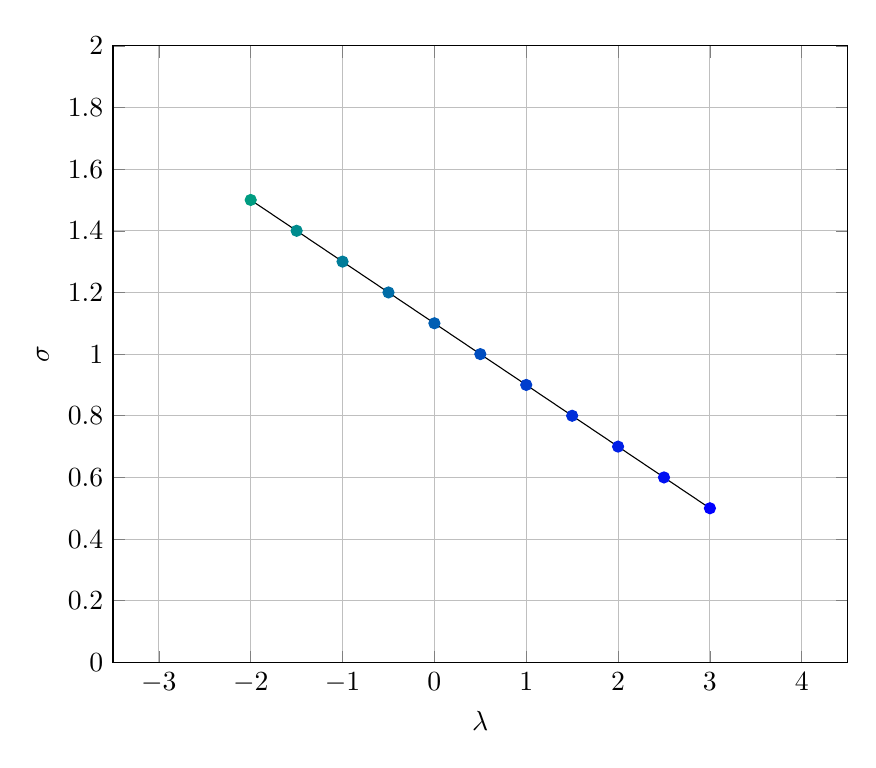
\begin{tikzpicture}[define rgb/.code={\definecolor{mycolor}{RGB}{#1}},
				rgb color/.style={define rgb={#1},mycolor}]
				
				\def\startlambda{-2}
				\def\endlambda{3}
				\def\startsigma{1.5}
				\def\endsigma{0.5}
				\def\steps{10}
				\definecolor{startcolor}{RGB}{0,156,129}
				\definecolor{endcolor}{RGB}{0,0,255}
				
				\begin{axis}[
					grid=major,
					xmax=4.5, ymax=2, xmin=-3.5, ymin=0,
					width=0.9\textwidth,
					xlabel={$\lambda$},
					ylabel={$\sigma$}
					]
					\draw (axis cs:-2, 1.5) -- (axis cs:3, 0.5);
					
					\addplot[rgb color={  0, 156, 129}, mark=*] coordinates {(-2  , 1.5)};
					\addplot[rgb color={  0, 140, 142}, mark=*] coordinates {(-1.5, 1.4)};
					\addplot[rgb color={  0, 125, 154}, mark=*] coordinates {(-1  , 1.3)};
					\addplot[rgb color={  0, 109, 167}, mark=*] coordinates {(-0.5, 1.2)};
					\addplot[rgb color={  0,  94, 179}, mark=*] coordinates {( 0  , 1.1)};
					\addplot[rgb color={  0,  78, 192}, mark=*] coordinates {( 0.5, 1.0)};
					\addplot[rgb color={  0,  62, 205}, mark=*] coordinates {( 1  , 0.9)};
					\addplot[rgb color={  0,  47, 217}, mark=*] coordinates {( 1.5, 0.8)};
					\addplot[rgb color={  0,  31, 230}, mark=*] coordinates {( 2  , 0.7)};
					\addplot[rgb color={  0,  16, 242}, mark=*] coordinates {( 2.5, 0.6)};
					\addplot[rgb color={  0,   0, 255}, mark=*] coordinates {( 3  , 0.5)};
				\end{axis}
			\end{tikzpicture}
			\caption{Subcaption of the left diagram.}
			\label{Fig:SubLeft}
		\end{subfigure}%
		~ 
		\begin{subfigure}[t]{0.5\textwidth}
			\centering
			\begin{tikzpicture}
				
				\def\startlambda{-2}
				\def\endlambda{3}
				\def\startsigma{1.5}
				\def\endsigma{0.5}
				\def\steps{10}
				\definecolor{startcolor}{RGB}{0,156,129}
				\definecolor{endcolor}{RGB}{0,0,255}
				
				\begin{axis}[
					grid=major,
					xmax=5, ymax=1, xmin=-5, ymin=0, samples=200,
					width=0.9\textwidth,
					xlabel={$x$},
					ylabel={$f_{\lambda,\sigma}(x)$}
					]
					\foreach [evaluate=\t as \v using (\t)*100/(\steps)] \t in {0,...,\steps}
					{
						\def\lambda{\startlambda + \t * (\endlambda - \startlambda) / \steps}
						\def\sigma{\startsigma + \t * (\endsigma - \startsigma) / \steps}
						
						\edef\temp{\noexpand
							\addplot[endcolor!\v!startcolor, thick]{gauss(x, \lambda, \sigma)};
							\noexpand}\temp
					}
				\end{axis}
			\end{tikzpicture}
			\caption{Subcaption of the right diagram.}
			\label{Fig:SubRight}
		\end{subfigure}
		\caption{Caption of both diagrams.}
		\label{Fig:Main1}
	\end{figure}

	\begin{figure}[H]
		\centering
		\begin{subfigure}[t]{0.5\textwidth}
			\centering
			\begin{tikzpicture}
				
				\definecolor{startcolor}{RGB}{0,156,129}
				\definecolor{endcolor}{RGB}{0,0,255}
				
				\begin{axis}[zmax=1,zmin=0,colormap={kit}{rgb255=(250,250,250) rgb255=(0,109,167)},grid=major,width=0.95\textwidth]
					\addplot3[color=endcolor,thick,samples y=0,samples=45,domain=-5:5] (x,5,{gauss(x,3,0.5)}) node[above, pos=0.6] {$f_{\nu}$}; 
					\addplot3[color=startcolor,thick,samples y=0,domain=-5:5] (-5,x,{gauss(x,-2,1.5)}) node[above, pos=0.6] {$f_{\mu}$}; 
					\addplot3[surf, domain=-5:5,domain y=-5:5] {gauss2d(x, y, 3, -2, 0.5, 1.5, -0.5)};  
				\end{axis}
			\end{tikzpicture}
			\caption{Subcaption of the diagram.}
			\label{Fig:Topleft}
		\end{subfigure}%
		~
		\begin{subfigure}[t]{0.5\textwidth}
			\centering
			\begin{tikzpicture}
				
				\definecolor{startcolor}{RGB}{0,156,129}
				\definecolor{endcolor}{RGB}{0,0,255}
				
				\begin{axis}[zmax=1,zmin=0,colormap={kit}{rgb255=(250,250,250) rgb255=(0,109,167)},grid=major,width=0.95\textwidth]
					\addplot3[color=endcolor,thick,samples y=0,samples=45,domain=-5:5] (x,5,{gauss(x,3,0.5)}) node[above, pos=0.6] {$f_{\nu}$}; 
					\addplot3[color=startcolor,thick,samples y=0,domain=-5:5] (-5,x,{gauss(x,-2,1.5)}) node[above, pos=0.6] {$f_{\mu}$}; 
					\addplot3[surf, domain=-5:5,domain y=-5:5] {gauss2d(x, y, 3, -2, 0.5, 1.5, 0)};  
				\end{axis}
			\end{tikzpicture}
			\caption{Subcaption of the diagram.}
			\label{Fig:TopRight}
		\end{subfigure}
	
		\vspace*{1em}
		
		\begin{subfigure}[t]{0.5\textwidth}
			\centering
			\begin{tikzpicture}
				
				\definecolor{startcolor}{RGB}{0,156,129}
				\definecolor{endcolor}{RGB}{0,0,255}
				
				\begin{axis}[zmax=1,zmin=0,colormap={kit}{rgb255=(250,250,250) rgb255=(0,109,167)},grid=major,width=0.95\textwidth]
					\addplot3[color=endcolor,thick,samples y=0,samples=45,domain=-5:5] (x,5,{gauss(x,3,0.5)}) node[above, pos=0.6] {$f_{\nu}$}; 
					\addplot3[color=startcolor,thick,samples y=0,domain=-5:5] (-5,x,{gauss(x,-2,1.5)}) node[above, pos=0.6] {$f_{\mu}$}; 
					\addplot3[surf, domain=-5:5,domain y=-5:5] {gauss2d(x, y, 3, -2, 0.5, 1.5, 0.5)};  
				\end{axis}
			\end{tikzpicture}
			\caption{Subcaption of the diagram.}
			\label{Fig:BotLeft}
		\end{subfigure}%
		~
		\begin{subfigure}[t]{0.5\textwidth}
			\centering
			\begin{tikzpicture}
				
				\definecolor{startcolor}{RGB}{0,156,129}
				\definecolor{endcolor}{RGB}{0,0,255}
				
				\begin{axis}[zmax=1,zmin=0,colormap={kit}{rgb255=(250,250,250) rgb255=(0,109,167)},grid=major,width=0.95\textwidth]
					\addplot3[color=endcolor,thick,samples y=0,samples=45,domain=-5:5] (x,5,{gauss(x,3,0.5)}) node[above, pos=0.6] {$f_{\nu}$}; 
					\addplot3[color=startcolor,thick,samples y=0,domain=-5:5] (-5,x,{gauss(x,-2,1.5)}) node[above, pos=0.6] {$f_{\mu}$}; 
					\addplot3[surf, domain=-5:5,domain y=-5:5] {gauss2d(x, y, 3, -2, 0.5, 1.5, 0.9)};  
				\end{axis}
			\end{tikzpicture}
			\caption{Subcaption of the diagram.}
			\label{Fig:BotRight}
		\end{subfigure}
		\caption{Caption of all diagrams.}
		\label{Fig:Main2}
	\end{figure}

	
	
	
\end{document}